
%(BEGIN_QUESTION)
% Copyright 2008, Tony R. Kuphaldt, released under the Creative Commons Attribution License (v 1.0)
% This means you may do almost anything with this work of mine, so long as you give me proper credit

Regn ut spenningen mellom punktene A og B i denne kretsen. (Vis alle utregninger)

$$\includegraphics[width=15.5cm]{i02527x01.eps}$$

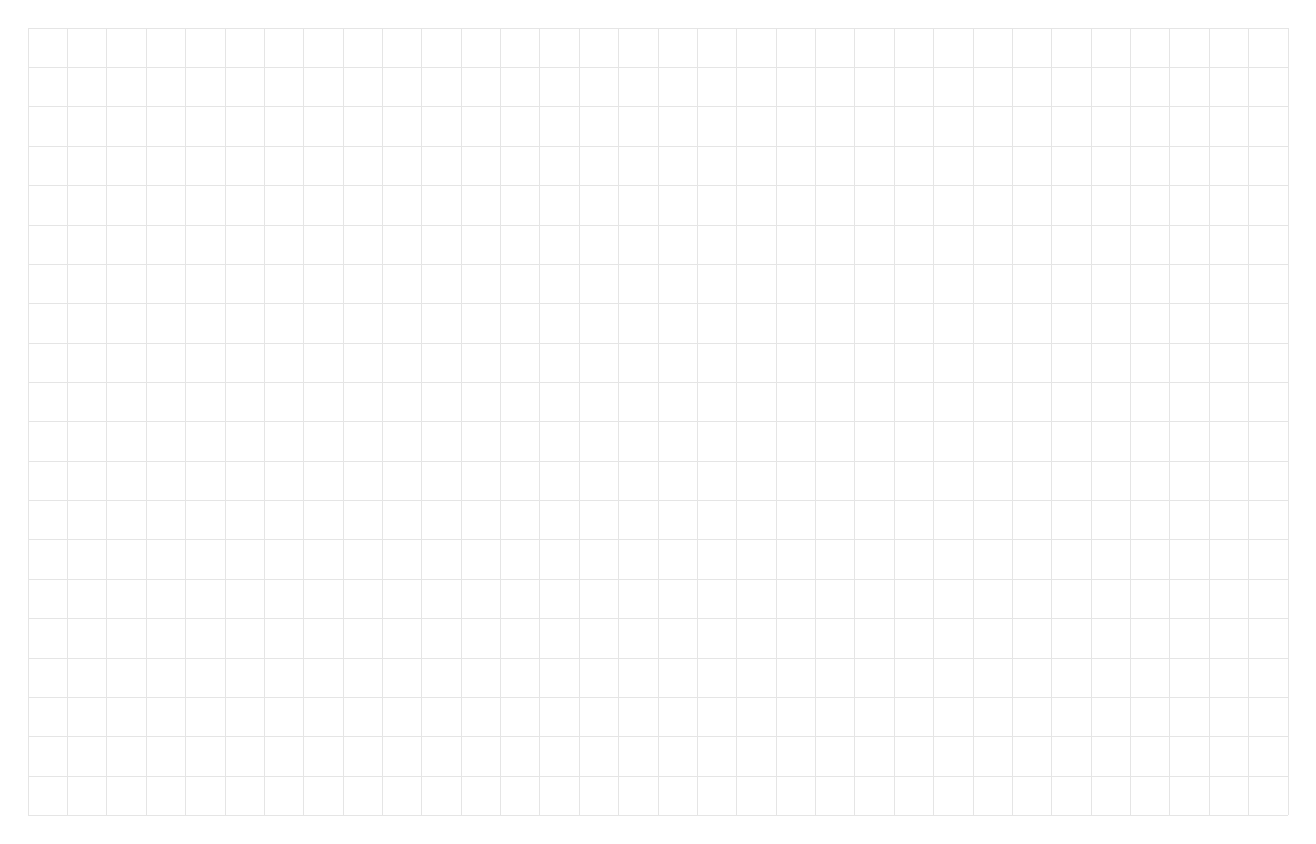
\begin{tikzpicture}
	\draw[step=0.5cm,gray!20,very thin]  grid (16,10) ;
\end{tikzpicture}
\underbar{file i02527}
%(END_QUESTION)





%(BEGIN_ANSWER)

$V_{\bf AB}$ = 9.198 volts, {\bf A} positive and {\bf B} negative.

$$\includegraphics[width=15.5cm]{i02527x02.eps}$$

The voltage between points A and B is the supply voltage (26 volts) minus the voltage drops across the 1k and parallel subnetwork resistors.  Alternatively, one could calculate $V_{AB}$ by adding the voltage drops of the 1k and 270 ohm resistors.

The latter solution makes it easiest to see the polarity of $V_{AB}$: noting how the voltage drops across the 1k and 270 ohm resistors are additive, we see point A being the most positive and point B being the most negative.

%(END_ANSWER)





%(BEGIN_NOTES)


%INDEX% Electronics review: Kirchhoff's Voltage Law (KVL)

%(END_NOTES)


